\chapter{Algorithmik}
\label{cha:algorithmik}
%Damit die mobilen Geräten den Nutzern Hinweise zum nächsten Notausgang geben können, müssen sie ihre eigene Position kennen. Daher soll ein dezentraler Lokalisierungsalgorithmus implementiert werden (siehe [2]). Beispielweise kann der minimale Nachrichten Hop-Count zu einem Notausgang im Zusammenhang mit der maximalen Kommunikationsreichweite zur Ap-proximation der Distanz des Knotens zum Ausgang dienen (siehe [1], gradient algorithm). Meh-rere (>=3) dieser Distanzen können wiederum zur Positionierung verwendet werden (Stichwort: Lateration. Siehe multilateration algorithm in [1] oder Bogenschnitt). In der Visualisierung sollte die Qualität der Positionierung erkennbar sein, d.h. es sollte zusätzlich zur wahren Position des Sensorknotens die errechnete Position erkennbar sein. 


\begin{figure}
\centering
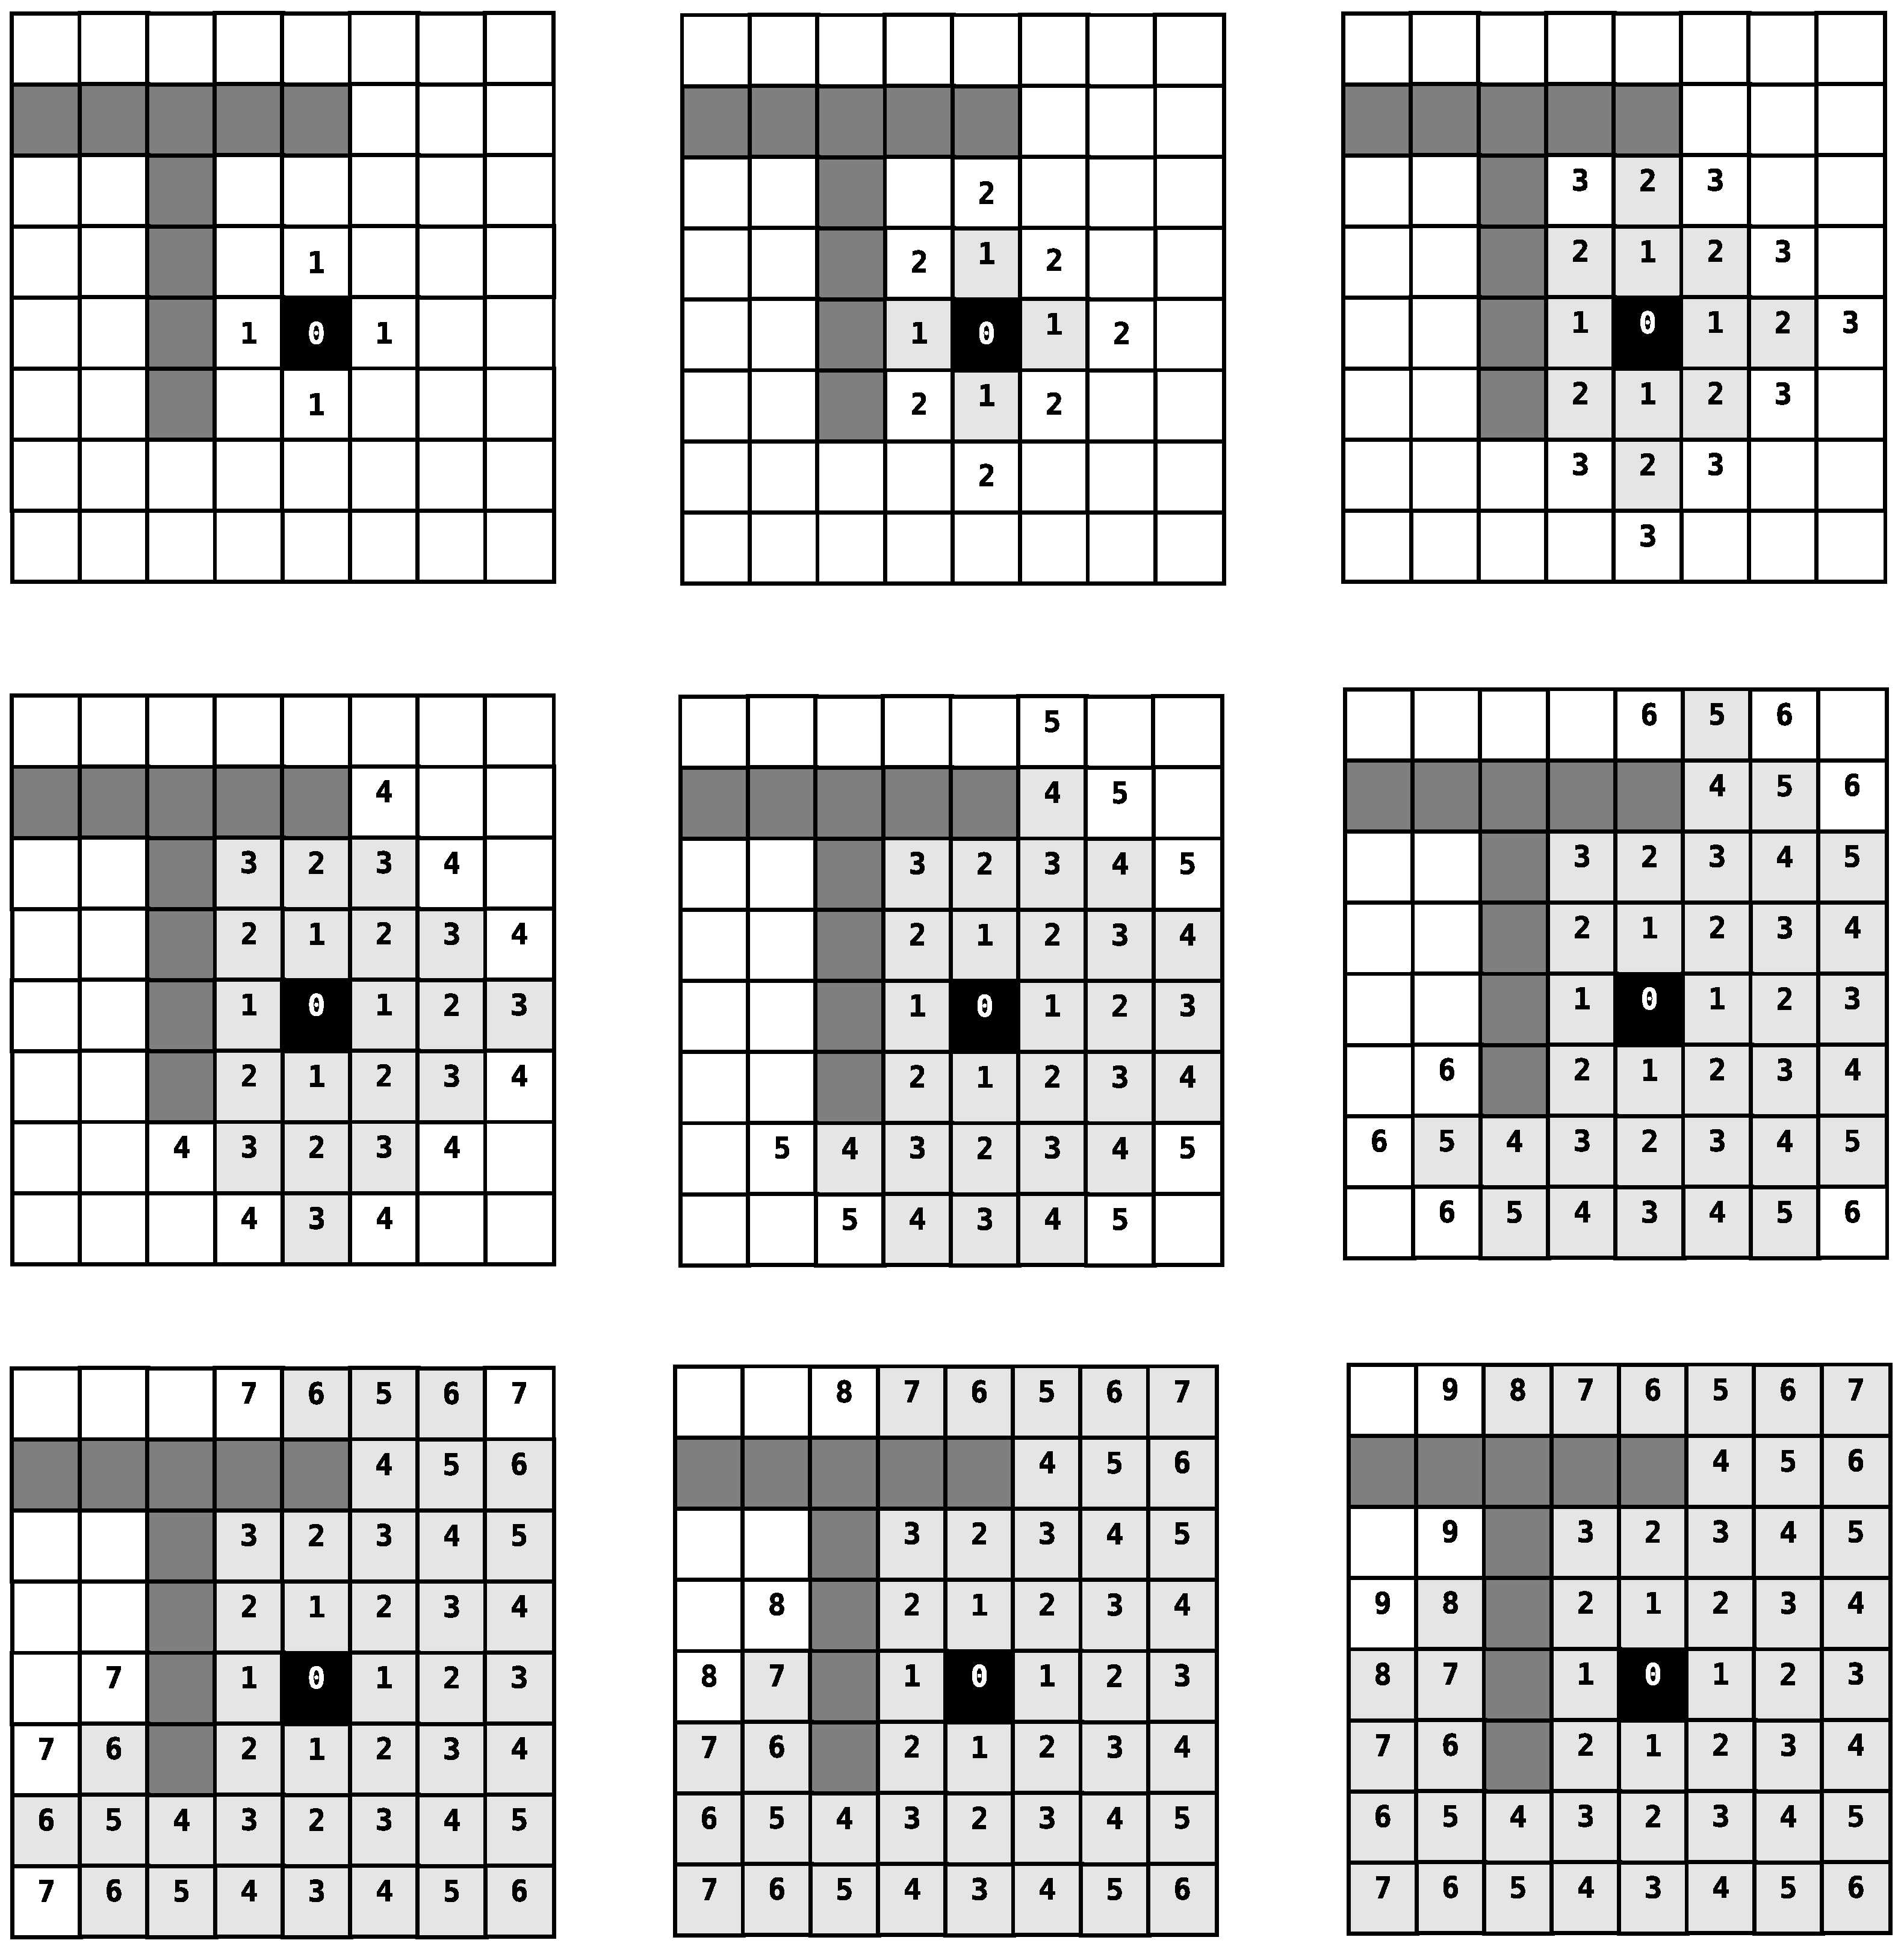
\includegraphics[height=0.9\textwidth]{algorithmik/flooding.eps}
\caption{Fluten der Patches (Zellulärer Automat)}
\label{fig:flooding}
\end{figure}